\documentclass{ximera}
\graphicspath{  %% When looking for images,
{./}            %% look here first,
{./pictures/}   %% then look for a pictures folder,
{../pictures/}  %% which may be a directory up.
{../../pictures/}  %% which may be a directory up.
{../../../pictures/}  %% which may be a directory up.
{../../../../pictures/}  %% which may be a directory up.
}

\usepackage{listings}
%\usepackage{circuitikz}
\usepackage{xcolor}
\usepackage{amsmath,amsthm}
\usepackage{subcaption}
\usepackage{graphicx}
\usepackage{tikz}
%\usepackage{tikz-3dplot}
\usepackage{amsfonts}
%\usepackage{mdframed} % For framing content
%\usepackage{tikz-cd}

  \renewcommand{\vector}[1]{\left\langle #1\right\rangle}
  \newcommand{\arrowvec}[1]{{\overset{\rightharpoonup}{#1}}}
  \newcommand{\ro}{\texttt{R}}%% row operation
  \newcommand{\dotp}{\bullet}%% dot product
  \renewcommand{\l}{\ell}
  \let\defaultAnswerFormat\answerFormatBoxed
  \usetikzlibrary{calc,bending}
  \tikzset{>=stealth}
  




%make a maroon color
\definecolor{maroon}{RGB}{128,0,0}
%make a dark blue color
\definecolor{darkblue}{RGB}{0,0,139}
%define the color fourier0 to be the maroon color
\definecolor{fourier0}{RGB}{128,0,0}
%define the color fourier1 to be the dark blue color
\definecolor{fourier1}{RGB}{0,0,139}
%define the color fourier 1t to be the light blue color
\definecolor{fourier1t}{RGB}{173,216,230}
%define the color fourier2 to be the dark green color
\definecolor{fourier2}{RGB}{0,100,0}
%define teh color fourier2t to be the light green color
\definecolor{fourier2t}{RGB}{144,238,144}
%define the color fourier3 to be the dark purple color
\definecolor{fourier3}{RGB}{128,0,128}
%define the color fourier3t to be the light purple color
\definecolor{fourier3t}{RGB}{221,160,221}
%define the color fourier0t to be the red color
\definecolor{fourier0t}{RGB}{255,0,0}
%define the color fourier4 to be the orange color
\definecolor{fourier4}{RGB}{255,165,0}
%define the color fourier4t to be the darker orange color
\definecolor{fourier4t}{RGB}{255,215,0}
%define the color fourier5 to be the yellow color
\definecolor{fourier5}{RGB}{255,255,0}
%define the color fourier5t to be the darker yellow color
\definecolor{fourier5t}{RGB}{255,255,100}
%define the color fourier6 to be the green color
\definecolor{fourier6}{RGB}{0,128,0}
%define the color fourier6t to be the darker green color
\definecolor{fourier6t}{RGB}{0,255,0}

%New commands for this doc for errors in copying
\newcommand{\eigenvar}{\lambda}
%\newcommand{\vect}[1]{\mathbf{#1}}
\renewcommand{\th}{^{\text{th}}}
\newcommand{\st}{^{\text{st}}}
\newcommand{\nd}{^{\text{nd}}}
\newcommand{\rd}{^{\text{rd}}}
\newcommand{\paren}[1]{\left(#1\right)}
\newcommand{\abs}[1]{\left|#1\right|}
\newcommand{\R}{\mathbb{R}}
\newcommand{\C}{\mathbb{C}}
\newcommand{\Hilb}{\mathbb{H}}
\newcommand{\qq}[1]{\text{#1}}
\newcommand{\Z}{\mathbb{Z}}
\newcommand{\N}{\mathbb{N}}
\newcommand{\q}[1]{\text{``#1''}}
%\newcommand{\mat}[1]{\begin{bmatrix}#1\end{bmatrix}}
\newcommand{\rref}{\text{reduced row echelon form}}
\newcommand{\ef}{\text{echelon form}}
\newcommand{\ohm}{\Omega}
\newcommand{\volt}{\text{V}}
\newcommand{\amp}{\text{A}}
\newcommand{\Seq}{\textbf{Seq}}
\newcommand{\Poly}{\textbf{P}}
\renewcommand{\quad}{\text{    }}
\newcommand{\roweq}{\simeq}
\newcommand{\rowop}{\simeq}
\newcommand{\rowswap}{\leftrightarrow}
\newcommand{\Mat}{\textbf{M}}
\newcommand{\Func}{\textbf{Func}}
\newcommand{\Hw}{\textbf{Hamming weight}}
\newcommand{\Hd}{\textbf{Hamming distance}}
\newcommand{\rank}{\text{rank}}
\newcommand{\longvect}[1]{\overrightarrow{#1}}
% Define the circled command
\newcommand{\circled}[1]{%
  \tikz[baseline=(char.base)]{
    \node[shape=circle,draw,inner sep=2pt,red,fill=red!20,text=black] (char) {#1};}%
}

% Define custom command \strikeh that just puts red text on the 2nd argument
\newcommand{\strikeh}[2]{\textcolor{red}{#2}}

% Define custom command \strikev that just puts red text on the 2nd argument
\newcommand{\strikev}[2]{\textcolor{red}{#2}}

%more new commands for this doc for errors in copying
\newcommand{\SI}{\text{SI}}
\newcommand{\kg}{\text{kg}}
\newcommand{\m}{\text{m}}
\newcommand{\s}{\text{s}}
\newcommand{\norm}[1]{\left\|#1\right\|}
\newcommand{\col}{\text{col}}
\newcommand{\sspan}{\text{span}}
\newcommand{\proj}{\text{proj}}
\newcommand{\set}[1]{\left\{#1\right\}}
\newcommand{\degC}{^\circ\text{C}}
\newcommand{\centroid}[1]{\overline{#1}}
\newcommand{\dotprod}{\boldsymbol{\cdot}}
%\newcommand{\coord}[1]{\begin{bmatrix}#1\end{bmatrix}}
\newcommand{\iprod}[1]{\langle #1 \rangle}
\newcommand{\adjoint}{^{*}}
\newcommand{\conjugate}[1]{\overline{#1}}
\newcommand{\eigenvarA}{\lambda}
\newcommand{\eigenvarB}{\mu}
\newcommand{\orth}{\perp}
\newcommand{\bigbracket}[1]{\left[#1\right]}
\newcommand{\textiff}{\text{ if and only if }}
\newcommand{\adj}{\text{adj}}
\newcommand{\ijth}{\emph{ij}^\text{th}}
\newcommand{\minor}[2]{M_{#2}}
\newcommand{\cofactor}{\text{C}}
\newcommand{\shift}{\textbf{shift}}
\newcommand{\startmat}[1]{
  \left[\begin{array}{#1}
}
\newcommand{\stopmat}{\end{array}\right]}
%a command to give a name to explorations and hints and theorems
\newcommand{\name}[1]{\begin{centering}\textbf{#1}\end{centering}}
\newcommand{\vect}[1]{\vec{#1}}
\newcommand{\dfn}[1]{\textbf{#1}}
\newcommand{\transpose}{\mathsf{T}}
\newcommand{\mtlb}[2][black]{\texttt{\textcolor{#1}{#2}}}
\newcommand{\RR}{\mathbb{R}} % Real numbers
\newcommand{\id}{\text{id}}
\newcommand{\coord}[1]{\langle#1\rangle}
\newcommand{\RREF}{\text{RREF}}
\newcommand{\Null}{\text{Null}}
\newcommand{\Nullity}{\text{Nullity}}
\newcommand{\Rank}{\text{Rank}}
\newcommand{\Col}{\text{Col}}
\newcommand{\Ef}{\text{EF}}
\newcommand{\boxprod}[3]{\abs{(#1\times#2)\cdot#3}}

\author{Zack Reed}
%borrowed from selinger linear algebra
\title{Centering Data for the SVD}
\begin{document}
\begin{abstract}

\end{abstract}
\maketitle


% ----------------------------------------------------------------------
\section*{Affine fitting}

So far, we have been looking to approximate a given collection of
points by a {\em subspace}, which necessarily passes through the
origin. But sometimes the points may not be near the origin, as in
this example:
\begin{center}
  \begin{tikzpicture}[baseline=-0.5ex, scale=0.8]
    \draw[thin,->] (-4,0) -- (4,0);
    \draw[thin,->] (0,-4) -- (0,4);
    % \draw[thick, blue] (0.91,1.76) +(-6,-6/-3.20) -- +(6,6/-3.20);
    \fill[color=red] (-0.54,2.53) circle (0.075);
    \fill[color=red] (4.26,0.53) circle (0.075);
    \fill[color=red] (-0.24,2.38) circle (0.075);
    \fill[color=red] (1.98,1.52) circle (0.075);
    \fill[color=red] (0.28,2.14) circle (0.075);
    \fill[color=red] (5.71,0.05) circle (0.075);
    \fill[color=red] (2.90,1.56) circle (0.075);
    \fill[color=red] (-3.21,2.97) circle (0.075);
    \fill[color=red] (5.44,-0.09) circle (0.075);
    \fill[color=red] (-0.37,1.87) circle (0.075);
    \fill[color=red] (-0.46,2.02) circle (0.075);
    \fill[color=red] (2.21,1.49) circle (0.075);
    \fill[color=red] (-0.91,2.23) circle (0.075);
    \fill[color=red] (0.81,1.80) circle (0.075);
    \fill[color=red] (0.47,1.91) circle (0.075);
    \fill[color=red] (0.96,2.34) circle (0.075);
    \fill[color=red] (-0.93,2.29) circle (0.075);
    \fill[color=red] (-0.35,2.09) circle (0.075);
    \fill[color=red] (1.99,1.11) circle (0.075);
    \fill[color=red] (2.34,1.31) circle (0.075);
    \fill[color=red] (-0.99,2.30) circle (0.075);
    \fill[color=red] (-2.26,2.78) circle (0.075);
    \fill[color=red] (4.07,0.84) circle (0.075);
    \fill[color=red] (0.50,2.19) circle (0.075);
    \fill[color=red] (-1.08,2.76) circle (0.075);
    \fill[color=red] (-0.10,2.07) circle (0.075);
    \fill[color=red] (1.49,1.46) circle (0.075);
    \fill[color=red] (2.05,1.08) circle (0.075);
    \fill[color=red] (4.18,0.74) circle (0.075);
    \fill[color=red] (0.29,1.98) circle (0.075);
    \fill[color=red] (-1.37,2.64) circle (0.075);
    \fill[color=red] (0.75,2.22) circle (0.075);
    \fill[color=red] (0.55,1.91) circle (0.075);
    \fill[color=red] (2.41,1.73) circle (0.075);
    \fill[color=red] (3.70,1.02) circle (0.075);
    \fill[color=red] (1.73,1.85) circle (0.075);
    \fill[color=red] (-0.03,1.99) circle (0.075);
    \fill[color=red] (2.60,1.00) circle (0.075);
    \fill[color=red] (-0.57,2.42) circle (0.075);
    \fill[color=red] (2.44,0.87) circle (0.075);
    \fill[color=red] (1.67,1.20) circle (0.075);
    \fill[color=red] (2.27,1.53) circle (0.075);
    \fill[color=red] (-1.48,2.27) circle (0.075);
    \fill[color=red] (-0.65,1.73) circle (0.075);
    \fill[color=red] (3.53,0.83) circle (0.075);
    \fill[color=red] (0.00,2.10) circle (0.075);
    \fill[color=red] (0.03,2.06) circle (0.075);
    \fill[color=red] (-0.40,2.34) circle (0.075);
    \fill[color=red] (0.48,1.91) circle (0.075);
    \fill[color=red] (-0.59,2.74) circle (0.075);
    \fill[color=red] (0.71,1.61) circle (0.075);
    \fill[color=red] (-0.04,1.88) circle (0.075);
    \fill[color=red] (0.33,1.89) circle (0.075);
    \fill[color=red] (4.66,0.67) circle (0.075);
    \fill[color=red] (3.68,1.23) circle (0.075);
    \fill[color=red] (1.06,1.51) circle (0.075);
    \fill[color=red] (-0.08,2.08) circle (0.075);
    \fill[color=red] (-0.24,1.75) circle (0.075);
    \fill[color=red] (4.36,0.91) circle (0.075);
    \fill[color=red] (1.17,1.51) circle (0.075);
    \fill[color=red] (1.25,2.07) circle (0.075);
    \fill[color=red] (2.36,1.48) circle (0.075);
    \fill[color=red] (-1.21,2.26) circle (0.075);
    \fill[color=red] (-0.13,1.83) circle (0.075);
    \fill[color=red] (1.23,1.51) circle (0.075);
    \fill[color=red] (2.30,1.40) circle (0.075);
    \fill[color=red] (-1.08,2.50) circle (0.075);
    \fill[color=red] (-1.62,2.33) circle (0.075);
    \fill[color=red] (-0.27,2.32) circle (0.075);
    \fill[color=red] (-1.75,2.52) circle (0.075);
    \fill[color=red] (3.37,1.10) circle (0.075);
    \fill[color=red] (-1.10,2.10) circle (0.075);
    \fill[color=red] (-0.54,1.85) circle (0.075);
    \fill[color=red] (2.16,1.16) circle (0.075);
    \fill[color=red] (-0.15,2.11) circle (0.075);
  \end{tikzpicture}
\end{center}
In this case, approximating the points by a subspace passing through
the origin does not make much sense. Instead, we should be looking for
an \textbf{affine subspace}. An affine subspace is similar to a
subspace, except it does not necessarily contain the origin.

You can analyze this data by loading \texttt{+linalg/subspace\_fitting\_affine\_data.mat} in MATLAB.

In fact, the \href{https://ximera.osu.edu/appliedlinearalgebra/c6ChapterSix/learningActivities/m6LearningActivities/leastSquares/leastSquaresApplicationVotingImages}{voting records example} required an accounting of this centering issue as well. We have centered many data sets before, in some ways this section is a deeper dive into the importance of centering data. 

The crux of the matter is that if data is not centered, the when the SVD is calculated, the directions of maximum spread are still calculated according to the origin, and hence the spread is misrepresented towards the cluster away from the origin, not allowing for the true spread of the data to be captured by the SVD. 


\begin{definition}\name{Affine subspace}\label{def:affine-subspace}

  Let $V$ be a vector space. A subset $A\subseteq V$ is called an
  \textbf{affine subspace} of $V$ if $A$ is either empty, or else of
  the form
  \begin{equation*}
    A = \vect{v} + W = \set{\vect{v}+\vect{w} \mid \vect{w}\in W},
  \end{equation*}
  where $\vect{v}\in V$ and $W$ is a subspace of\/ $V$.

  In other words, an affine subspace has been shifted by some vector $\vec{v}$.
\end{definition}

The set in the previous figure is centered around the point $\begin{bmatrix}
  .9065\\1.7625
\end{bmatrix}$, as seen in the following figure:

\begin{center}
  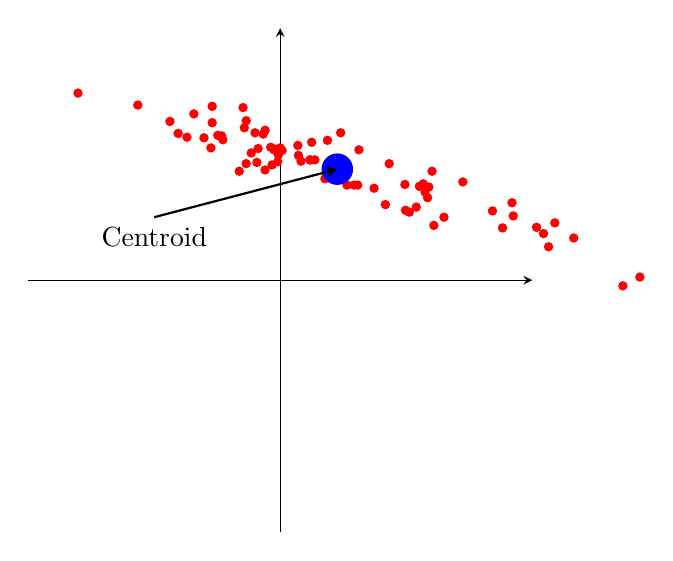
\begin{tikzpicture}[baseline=-0.5ex, scale=0.8]
    \draw[thin,->] (-4,0) -- (4,0);
    \draw[thin,->] (0,-4) -- (0,4);
    % \draw[thick, blue] (0.91,1.76) +(-6,-6/-3.20) -- +(6,6/-3.20);
    \fill[color=red] (-0.54,2.53) circle (0.075);
    \fill[color=red] (4.26,0.53) circle (0.075);
    \fill[color=red] (-0.24,2.38) circle (0.075);
    \fill[color=red] (1.98,1.52) circle (0.075);
    \fill[color=red] (0.28,2.14) circle (0.075);
    \fill[color=red] (5.71,0.05) circle (0.075);
    \fill[color=red] (2.90,1.56) circle (0.075);
    \fill[color=red] (-3.21,2.97) circle (0.075);
    \fill[color=red] (5.44,-0.09) circle (0.075);
    \fill[color=red] (-0.37,1.87) circle (0.075);
    \fill[color=red] (-0.46,2.02) circle (0.075);
    \fill[color=red] (2.21,1.49) circle (0.075);
    \fill[color=red] (-0.91,2.23) circle (0.075);
    \fill[color=red] (0.81,1.80) circle (0.075);
    \fill[color=red] (0.47,1.91) circle (0.075);
    \fill[color=red] (0.96,2.34) circle (0.075);
    \fill[color=red] (-0.93,2.29) circle (0.075);
    \fill[color=red] (-0.35,2.09) circle (0.075);
    \fill[color=red] (1.99,1.11) circle (0.075);
    \fill[color=red] (2.34,1.31) circle (0.075);
    \fill[color=red] (-0.99,2.30) circle (0.075);
    \fill[color=red] (-2.26,2.78) circle (0.075);
    \fill[color=red] (4.07,0.84) circle (0.075);
    \fill[color=red] (0.50,2.19) circle (0.075);
    \fill[color=red] (-1.08,2.76) circle (0.075);
    \fill[color=red] (-0.10,2.07) circle (0.075);
    \fill[color=red] (1.49,1.46) circle (0.075);
    \fill[color=red] (2.05,1.08) circle (0.075);
    \fill[color=red] (4.18,0.74) circle (0.075);
    \fill[color=red] (0.29,1.98) circle (0.075);
    \fill[color=red] (-1.37,2.64) circle (0.075);
    \fill[color=red] (0.75,2.22) circle (0.075);
    \fill[color=red] (0.55,1.91) circle (0.075);
    \fill[color=red] (2.41,1.73) circle (0.075);
    \fill[color=red] (3.70,1.02) circle (0.075);
    \fill[color=red] (1.73,1.85) circle (0.075);
    \fill[color=red] (-0.03,1.99) circle (0.075);
    \fill[color=red] (2.60,1.00) circle (0.075);
    \fill[color=red] (-0.57,2.42) circle (0.075);
    \fill[color=red] (2.44,0.87) circle (0.075);
    \fill[color=red] (1.67,1.20) circle (0.075);
    \fill[color=red] (2.27,1.53) circle (0.075);
    \fill[color=red] (-1.48,2.27) circle (0.075);
    \fill[color=red] (-0.65,1.73) circle (0.075);
    \fill[color=red] (3.53,0.83) circle (0.075);
    \fill[color=red] (0.00,2.10) circle (0.075);
    \fill[color=red] (0.03,2.06) circle (0.075);
    \fill[color=red] (-0.40,2.34) circle (0.075);
    \fill[color=red] (0.48,1.91) circle (0.075);
    \fill[color=red] (-0.59,2.74) circle (0.075);
    \fill[color=red] (0.71,1.61) circle (0.075);
    \fill[color=red] (-0.04,1.88) circle (0.075);
    \fill[color=red] (0.33,1.89) circle (0.075);
    \fill[color=red] (4.66,0.67) circle (0.075);
    \fill[color=red] (3.68,1.23) circle (0.075);
    \fill[color=red] (1.06,1.51) circle (0.075);
    \fill[color=red] (-0.08,2.08) circle (0.075);
    \fill[color=red] (-0.24,1.75) circle (0.075);
    \fill[color=red] (4.36,0.91) circle (0.075);
    \fill[color=red] (1.17,1.51) circle (0.075);
    \fill[color=red] (1.25,2.07) circle (0.075);
    \fill[color=red] (2.36,1.48) circle (0.075);
    \fill[color=red] (-1.21,2.26) circle (0.075);
    \fill[color=red] (-0.13,1.83) circle (0.075);
    \fill[color=red] (1.23,1.51) circle (0.075);
    \fill[color=red] (2.30,1.40) circle (0.075);
    \fill[color=red] (-1.08,2.50) circle (0.075);
    \fill[color=red] (-1.62,2.33) circle (0.075);
    \fill[color=red] (-0.27,2.32) circle (0.075);
    \fill[color=red] (-1.75,2.52) circle (0.075);
    \fill[color=red] (3.37,1.10) circle (0.075);
    \fill[color=red] (-1.10,2.10) circle (0.075);
    \fill[color=red] (-0.54,1.85) circle (0.075);
    \fill[color=red] (2.16,1.16) circle (0.075);
    \fill[color=red] (-0.15,2.11) circle (0.075);
    \fill[color=blue] (.9065,1.7625) circle (.25);
    \draw[thick, ->] (-2,1) -- (.9065,1.7625) node[pos=0, below] {Centroid};
  \end{tikzpicture}
\end{center}

We call the vector $\vec{v}$ around which any affine space is centered the \emph{centroid}.

\begin{definition}\name{Centroid}\label{def:centroid}
  Given $m$ vectors $\vect{v}_1,\ldots,\vect{v}_m$, their
  \textbf{centroid}is the vector
  \begin{equation*}
    \centroid{\vect{v}} = \frac{1}{m}(\vect{v}_1+\ldots+\vect{v}_m).
  \end{equation*}
  It is also sometimes called the \textbf{average} or the \textbf{center of mass} of the vectors.
\end{definition}

\begin{proposition}\name{Solution of the affine subspace fitting problem}\label{prop:affine-subspace-fitting}
  Given vectors $\vect{v}_1,\ldots,\vect{v}_m\in\R^n$ and $k\leq n$,
  the optimal solution to the affine subspace fitting problem can be
  computed as follows:
  \begin{enumerate}
  \item Compute the centroid $\centroid{\vect{v}} =
    \frac{1}{m}(\vect{v}_1+\ldots+\vect{v}_m)$ of the vectors.
  \item Let $\vect{w}_i = \vect{v}_i - \centroid{\vect{v}}$, for all
    $i=1,\ldots,n$.
  \item Use the SVD to find the best-fitting subspace $W$ for the centered subspace.
  \item If desired, shift $W$ by $centroid{\vec{v}}$ to create an affine solutinon subspace.
  \end{enumerate}
  Then the best solution to the affine subspace problem is
  $\centroid{\vect{v}} + W$.
\end{proposition}

\begin{example}\name{Affine subspace fitting problem}\label{ex:affine-subspace-fitting}
  Consider the following collection of points in $\R^2$:
  \begin{equation*}
    \set{
      \startmat{r} 10 \\ -6 \stopmat,
      \startmat{r} 2 \\ 10 \stopmat,
      \startmat{r} 5 \\ -1 \stopmat,
      \startmat{r} 8 \\ 3 \stopmat,
      \startmat{r} 2 \\ 5 \stopmat,
      \startmat{r} 3 \\ 3 \stopmat,
      \startmat{r} 4 \\ 11 \stopmat,
      \startmat{r} 10 \\ -1 \stopmat,
      \startmat{r} 1 \\ 12 \stopmat
    }.
  \end{equation*}
  Find the 1-dimensional affine subspace that best approximates this
  collection of points. What is the total squared distance of the
  points to the subspace?

  \textbf{Solution:}

  We start by computing the centroid:


  \begin{equation*}
    \centroid{\vect{v}} =
    \frac{1}{9}(\vect{v}_1+\ldots+\vect{v}_9)
    = \frac{1}{9}\startmat{r} 45 \\ 36 \stopmat
    = \startmat{r} \answer{5} \\ \answer{4} \stopmat.
  \end{equation*}

  Next, we shift all vectors by $-\centroid{\vect{v}}$ to get a new
  collection of vectors $\vect{w}_1,\ldots,\vect{w}_9$ centered at the
  origin.
  For example,

  \begin{eqnarray*}
    \vect{w}_1 ~~=~~ \vect{v}_1 - \centroid{\vect{v}}
    &=& \startmat{r} 10 \\ -6 \stopmat
    - \startmat{r} 5 \\ 4 \stopmat
    ~~=~~ \startmat{r} 5 \\ -10 \stopmat,
    \\
    \vect{w}_2 ~~=~~ \vect{v}_2 - \centroid{\vect{v}}
    &=& \startmat{r} 2 \\ 10 \stopmat
    - \startmat{r} 5 \\ 4 \stopmat
    ~~=~~ \startmat{r} -3 \\ 6 \stopmat,
  \end{eqnarray*}

  and so on. We get

  \begin{equation*}
    \set{\vect{w}_1,\ldots,\vect{w}_9} =
    \set{
      \startmat{r} \answer{5} \\ -10 \stopmat,
      \startmat{r} -3 \\ \answer{6} \stopmat,
      \startmat{r} \answer{0} \\ -5 \stopmat,
      \startmat{r} 3 \\ \answer{-1} \stopmat,
      \startmat{r} \answer{-3} \\ 1 \stopmat,
      \startmat{r} -2 \\ \answer{-1} \stopmat,
      \startmat{r} \answer{-1} \\ 7 \stopmat,
      \startmat{r} 5 \\ \answer{-5} \stopmat,
      \startmat{r} -4 \\ \answer{8} \stopmat
    }.
  \end{equation*}

  Next we, we use the SVD. 
  
  In the code below, the centering is done by the code \texttt{W-mean(W,2)*ones(1,9)}, which turns the single vector \texttt{mean(W,2)} into a $2\times 9$ matrix of the centroid repeated 9 times.
  
  \begin{verbatim}
  
    W=[10 2 5 8 2 3 4 10 1;
    -6 10 -1 3 5 3 11 -1 12];
    W_centered=W-mean(W,2)*ones(1,9);
    [U, S, V]=svd(W_centered)

  \end{verbatim}

  We get the left singular vectors 

  $U=\begin{bmatrix}
    \answer[tolerance=.01]{.4472}&\answer[tolerance=.01]{.8944}\\\answer[tolerance=.01]{-.8944}&\answer[tolerance=.01]{.4472}
  \end{bmatrix}$ and $S=\begin{bmatrix}\answer[tolerance=.01]{19.2354}&0\\0&\answer[tolerance=.01]{5.4772}\end{bmatrix}$. You might notice that $S$ is really a $\answer{2}\times \answer{9}$ matrix, and that $V$ is a $\answer{9}\times \answer{9}$ matrix. This is because the domain of $W$ as a linear transformation is $\RR^9$, and also because there are $\answer{9}$ data vectors.

  We interpret this to mean that in $\RR^2$, the data is most spread in the direction $\vec{u}_1=\begin{bmatrix}
    \answer[tolerance=.01]{.4472}\\ \answer[tolerance=.01]{-.8944}
  \end{bmatrix}$ in the amount $\sigma_1=\answer[tolerance=.01]{19.2354}$. 
  
  We form a line from the first singular vector, offset by the centroid, 
  to make the best-fitting 1-dimensional affine subspace for
  $\vect{v}_1,\ldots,\vect{v}_9$, 
  \begin{equation*}
    \centroid{\vect{v}} + W
    = \set{\centroid{\vect{v}} + \vect{w} \mid \vect{w}\in W}
    = \set{\startmat{r} \answer{5} \\ \answer{4} \stopmat +
        t\startmat{r} .4472 \\ -.8944 \stopmat ~\text{ such that }~ t\in\R}.
  \end{equation*}

  Note that this is the equation of a line passing through the
  centroid $\centroid{\vect{v}}$, and with direction vector
  $\vect{u}_1$. The points $\vect{v}_1,\ldots,\vect{v}_9$, their
  centroid, and the affine subspace $\centroid{\vect{v}} + W$ are
  shown in the following illustration:
  \begin{center}
    \begin{tikzpicture}[scale=0.2]
      \draw[thin,->] (-12,0) -- (12,0);
      \draw[thin,->] (0,-12) -- (0,12);
      \draw[thin] (0,10) -- (-1,10) node[left] {$10$};
      \draw[thin] (10,0) -- (10,-1) node[below] {$10$};
      \draw[thick,blue] (5,4) +(-6,12) -- +(6,-12);
      \fill[color=blue] (5,4) circle (0.6);
      \draw[blue, ->] (5,4) +(8,4) node[right,yshift=4] {centroid} -- +(0.4,0.2);
      \fill[color=red] (10, -6) circle (0.3);
      \fill[color=red] (10, -1) circle (0.3);
      \fill[color=red] (5, -1) circle (0.3);
      \fill[color=red] (8, 3) circle (0.3);
      \fill[color=red] (3, 3) circle (0.3);
      \fill[color=red] (2, 5) circle (0.3);
      \fill[color=red] (2, 10) circle (0.3);
      \fill[color=red] (4, 11) circle (0.3);
      \fill[color=red] (1, 12) circle (0.3);
    \end{tikzpicture}
  \end{center}
  \vspace{-4ex}\par  


We can also project the data onto the line to view the spread-maximizing projections:

\begin{verbatim}
  
  dots=U(:,1)'*W
  projections=U(:,1)*dots+[5;4]

\end{verbatim}

\begin{center}
  \begin{tikzpicture}[scale=0.2]
    \draw[thin,->] (-12,0) -- (12,0);
    \draw[thin,->] (0,-12) -- (0,12);
    \draw[thin] (0,10) -- (-1,10) node[left] {$10$};
    \draw[thin] (10,0) -- (10,-1) node[below] {$10$};
    \draw[thick,blue] (5,4) +(-6,12) -- +(6,-12);
    \fill[color=blue] (5,4) circle (0.6);
    \draw[blue, ->] (5,4) +(8,4) node[right,yshift=4] {centroid} -- +(0.4,0.2);
    \fill[color=red] (10, -6) circle (0.3);
    \fill[color=red] (10, -1) circle (0.3);
    \fill[color=red] (5, -1) circle (0.3);
    \fill[color=red] (8, 3) circle (0.3);
    \fill[color=red] (3, 3) circle (0.3);
    \fill[color=red] (2, 5) circle (0.3);
    \fill[color=red] (2, 10) circle (0.3);
    \fill[color=red] (4, 11) circle (0.3);
    \fill[color=red] (1, 12) circle (0.3);

        % Bright purple dots from data
    \fill[color=purple] (10,-6) circle (0.4);
    \fill[color=purple] (2,10) circle (0.4);
    \fill[color=purple] (7,0) circle (0.4);
    \fill[color=purple] (6,2) circle (0.4);
    \fill[color=purple] (4,6) circle (0.4);
    %\fill[color=purple] (5,4) circle (0.4);
    \fill[color=purple] (2,10) circle (0.4); % Duplicate from data
    \fill[color=purple] (8,-2) circle (0.4);
    \fill[color=purple] (1,12) circle (0.4);
  \end{tikzpicture}
\end{center}
\vspace{-4ex}\par  

\end{example}

The plots from \href{https://ximera.osu.edu/appliedlinearalgebra/c6ChapterSix/learningActivities/m6LearningActivities/leastSquares/leastSquaresApplicationVotingImages}{voting records example} were exactly the projections of the voting data onto the centered $1D$ and $2D$ best-fitting subspaces formed from the SVD. 

The singular vectors that form these subspaces are often called \emph{principal components}. This same kind of subspace-fitting method takes many names depening on the STEM domain, but you will often hear \emph{principa component analysis} (data science/statistics) or \emph{proper orthogonal decomposition} (applied mathematics).

\end{document}